\documentclass[twoside, 10pt]{article}

% Українська версія статті noether_casimir_drive.tex.

\usepackage[T1, T2A]{fontenc}   % Standard package for selecting font encodings
\usepackage[utf8]{inputenc} % Accept different input encodings
\usepackage[english, russian, ukrainian]{babel}

\usepackage{mathptmx}

\usepackage{indentfirst}    % Indent first paragraph after section header

\usepackage{sectsty}        % Control sectional headers

\sectionfont{\normalfont\Large\textbf}
\subsectionfont{\normalfont\large\textbf}

\usepackage{multicol}       % Intermix single and multiple columns
\usepackage{orcidlink}      % Insert hyperlinked ORCiD logo
\usepackage{fancyhdr}       % Extensive control of page headers and footers

\usepackage{filecontents}
\usepackage{hyperref, doi}
\usepackage[numbers]{natbib}

\bibliographystyle{myunsrtnat}

% --- METADATA ---
\def\myfirstpage{1}
\def\mylastpage{15}
\def\mypages{\myfirstpage-\mylastpage}
\def\myfilename{noether_casimir_drive_uk_v2}
\def\myname{О. Дроздов}
\def\mynameukr{О. Дроздов}
\def\mytitle{Теорема Нетер та стільниковий рушій Казимира: про незбереження імпульсу в асиметричних вакуумних системах}
\def\mytitleukr{Теорема Нетер та стільниковий рушій Казимира: про незбереження імпульсу в асиметричних вакуумних системах}
\def\myissn{2222-5617}
\def\mydoi{10.26565/2222-5617-2026-XX-XX} % ← placeholder, замените при подаче
\def\myemail{alexey.drozdov.07@gmail.com}
\def\ukrvisnyk{Вісник Харківського національного університету імені В.~Н.~Каразіна, серія «Фізика», вип. XX, \mypages~(2026)}
\def\envisnyk{The Journal of V.~N.~Karazin Kharkiv National University. Series “Physics” Iss. XX, \mypages~(2026)}
\def\ruvisnyk{Вестник Харьковского национального университета имени В.~Н.~Каразина, серия «Физика», вып. XX, \mypages~(2026)}
\def\myworkplace{Харківський національний університет імені В.~Н.~Каразіна, майдан Свободи, 4, 61022 Харків, Україна}
\def\myworkplaceukr{Харківський національний університет імені В.~Н.~Каразіна, майдан Свободи, 4, 61022 Харків, Україна}
\def\mynameen{A. Drozdov}
\def\mytitleen{Noether's theorem and the Casimir honeycomb drive: on non-conservation of momentum in asymmetric vacuum systems}
\def\myworkplaceen{V.~N.~Karazin Kharkiv National University, 61022, 4 Svoboda Sq., Kharkiv, Ukraine}
\def\myreceiveden{Received on January 9, 2026.}
\def\myaccepteden{Accepted for publication on January 9, 2026.}
\def\myorcidlink{0009-0004-1386-4534}

\def\myreceived{Надійшла до редакції 9 січня 2026 р.}
\def\myaccepted{Прийнято до друку 9 січня 2026 р.}
\def\myreceivedukr{Надійшла до редакції 9 січня 2026 р.}
\def\myacceptedukr{Прийнято до друку 9 січня 2026 р.}

\def\licenseref{http://creativecommons.org/licenses/by/4.0/}

\def\myvspacebeforesubsection{-2.0mm}
\def\myvspaceaftersubsection{-2.5mm}

\def\collontitulasfontcode{lmss}

\newcommand{\MyTitle}{\expandafter\MakeUppercase\expandafter{\mytitle}}
\newcommand{\MyTitleUkr}{\expandafter\MakeUppercase\expandafter{\mytitleukr}}

\fancypagestyle{firstpagestyle}{
\renewcommand{\headrulewidth}{0.6pt}
\fancyhead[C]{\ukrvisnyk \\ \envisnyk}
\renewcommand{\footrulewidth}{0.6pt}
\fancyfoot[L]{\footbox{${}^{\copyright}$ \myname}}
\fancyfoot[R]{\footbox[r]{\fontencoding{T1}\fontfamily{\collontitulasfontcode}\selectfont \textit{Open Access. This article is licensed under a Creative Commons Attribution 4.0} \\
\href{\licenseref}{\textit{\licenseref}}}}
}

\usepackage{graphicx}
\usepackage{caption}
\DeclareCaptionFormat{nocaption}{}
\captionsetup{format=nocaption,aboveskip=0pt,belowskip=0pt}
\usepackage{float}
\floatplacement{figure}{H}
\usepackage{xcolor}
\usepackage{enumerate}
\usepackage{geometry}
\usepackage{amsmath, amssymb}
\usepackage{textcomp}
\usepackage{upquote}
\usepackage{ucs}
\usepackage{grffile}
\usepackage[Export]{adjustbox}
\adjustboxset{max size={0.9\linewidth}{0.9\paperheight}}
\usepackage{longtable, booktabs, enumitem, ulem, wrapfig, sidecap}

\providecommand{\keywords}[1]{\textbf{\textit{Ключові слова:}} #1}
\providecommand{\keywordsukr}[1]{\textbf{Ключові слова:} #1}

\author{\myname \,\orcidlink{\myorcidlink}}
\title{\textbf{\MyTitle.}}
\date{}

\definecolor{urlcolor}{rgb}{0,.145,.698}
\definecolor{linkcolor}{rgb}{0,0,0}
\definecolor{citecolor}{rgb}{0,0,0}

\providecommand{\doi}[1]{DOI: \href{https://doi.org/#1}{#1}}

\geometry{verbose,a4paper,includehead,includefoot,
nomarginpar,
headheight=26pt,footskip=58pt,
tmargin=1.1cm,bmargin=1.0cm,lmargin=1.85cm,rmargin=1.85cm}
% Многострочные колонтитулы: \footbox выравнивает блок по нижней строке, поэтому он растёт
% вверх от базовой линии footskip и не уходит за край листа; footskip (58pt) больше высоты
% четырёх строк \scriptsize, поэтому текст на колонтитул не наезжает.
\newcommand{\footbox}[2][l]{\parbox[b]{0.88\linewidth}{\scriptsize\if#1r\raggedleft\else\raggedright\fi #2}}

\setlength{\columnsep}{0.5cm}

% forbid word transfer
\hyphenpenalty=10000

\begin{document}

\fontencoding{T2A}\fontfamily{ptm}\selectfont

\setcounter{page}{\myfirstpage}

\pagestyle{fancy}
\fancyhead{}
\fancyhead[CE]{\fontencoding{T2A}\fontfamily{ptm}{\selectfont \textit{\mytitle.}}}
\fancyhead[CO]{\fontencoding{T2A}\fontfamily{ptm}{\selectfont \textit{\myname}}}
\renewcommand{\headrulewidth}{0.6pt}
\fancyfoot{}
\fancyfoot[LE,RO]{\thepage}
\fancyfoot[LO]{\footbox{{\fontencoding{T2A}\fontfamily{ptm}\selectfont \ukrvisnyk} \\ {\fontencoding{T1}\fontfamily{\collontitulasfontcode}\selectfont \envisnyk}}}
\fancyfoot[RE]{\footbox[r]{{\fontencoding{T2A}\fontfamily{ptm}\selectfont \ukrvisnyk} \\ {\fontencoding{T1}\fontfamily{\collontitulasfontcode}\selectfont \envisnyk}}}
\fancyfoot[CO,CE]{}

$\,$

\thispagestyle{firstpagestyle}

\vspace{-9.4mm}

\begin{tabular}{lcr}
\doi{\mydoi}
& \,\,\,\,\,\,\,\,\,\,\,\,\,\, \,\,\,\,\,\,\,\,\,\,\,\,\,\, \,\,\,\,\,\,\,\,\,\,\,\,\,\, \,\,\,\,\,\,\,\,\,\,\,\,\,\, \,\,\,\,\,\,\,\,\,\,\,\,\,\, \,\,\,\,\,\,\,\,\,\,\,\,\,\,
& ISSN \myissn (Print)
\end{tabular}

\vspace{9mm}

\begin{tabular}{l}
Оригінальна стаття \\
Стаття в друці \\
\href{https://doi.org/\mydoi}{https://doi.org/\mydoi} \\
УДК 53.09, 621.3, 629.7 \\
PACS: 11.10.Ef, 03.70.+k, 42.50.Lc \\
\end{tabular}

\section*{\centering {\fontencoding{T2A}\fontfamily{ptm}{\selectfont \MyTitle}}}

\vspace{7mm}
\centerline{\Large{\myname \,\orcidlink{\myorcidlink} }}
\vspace{7.5mm}
\centerline{\textit{\myworkplace}}
\centerline{\textit{E-mail: \href{mailto:\myemail}{\myemail}}}

\vspace{5mm}
\centerline{\myreceived}
\centerline{\myaccepted}

\vspace{5mm}

Стільниковий рушій Казимира \cite{Drozdov2024} --- ідеально провідна пластина з нанорозмірною
стільниковою структурою з одного боку --- розглядається з погляду симетрій. Через асиметрію
вакуумних мод з двох боків пластини система не є інваріантною відносно трансляцій уздовж нормалі:
вакуумний гамільтоніан явно залежить від координати \(l\), і за теоремою Нетер імпульс поля вздовж
цієї осі не зберігається. Сила тяги дорівнює \(\partial\langle H\rangle/\partial l\). Потім ту саму
силу обчислено незалежно --- через тензор натягів Максвелла, побудований з полів власних мод
резонатора. Помодово обидва виведення збігаються тотожно (теорема Гельмана--Фейнмана), а після
регуляризації --- у границі \(ak_m\to\infty\). Попутно знайдено й виправлено помилку в додатку~B
роботи \cite{Drozdov2024}: для TM-мод відношення тиску до густини енергії дорівнює \(k_z^2/k^2\),
а не одиниці. Тензорний розрахунок показує, де прикладена сила: це стрибок \(\langle T_{zz}\rangle\)
на поверхні металу, і тому потік імпульсу через будь-яку замкнену вакуумну поверхню, що охоплює
пластину, не залежить від положення її граней. Нарешті, показано, що стандартний баланс імпульсу
(\S\,105 Тамма) при \(\langle\mathbf S\rangle=0\) втрачає саме ці стрибкові члени. Не зберігається
імпульс поля (і пластини); повний імпульс системи \emph{пластина\,+\,поле\,+\,опора} зберігається.

\vspace{5mm}

\noindent
\begin{keywords}
\textit{теорема Нетер, ефект Казимира, квантовий вакуум, незбереження імпульсу, тензор натягів Максвелла, наностільники, тяга Казимира}
\end{keywords}

\vspace{5mm}

\noindent
\textbf{Як цитувати}: \textit{\mynameukr}. \textit{\mytitleukr}. {\ukrvisnyk}. \href{https://doi.org/\mydoi} {https://doi.org/\mydoi}.

\vspace{5mm}

\noindent
\textbf{In cites}: \textit{\mynameen}. \textit{\mytitleen}. {\envisnyk}. \href{https://doi.org/\mydoi} {https://doi.org/\mydoi}.

\vspace{5mm}

\newpage

\begin{multicols}{2}

\vspace{\myvspacebeforesubsection}
\subsection*{\centering{\fontencoding{T2A}\fontfamily{ptm}{\selectfont ВСТУП}}}
\vspace{\myvspaceaftersubsection}


У роботі \cite{Drozdov2024} показано, що ідеально провідна пластина, один бік якої гладкий, а
другий вкритий стільниками з квадратною коміркою \(a\times a\), зазнає з боку електромагнітного
вакууму результуючої сили. Силу обчислено як різницю густин енергії нульових коливань з двох боків
пластини, регуляризовану за формулою Ейлера--Маклорена; для комірки \(a\approx2\)~мкм вона
виявилася порядку кількох дин на квадратний метр.

Такий результат неминуче викликає запитання: як однотільна сила сумісна зі збереженням імпульсу?
У класичній конфігурації Казимира з двома пластинами сили, що діють на пластини, рівні й
протилежні, і запитання не виникає. Тут другого тіла немає.

Ця робота відповідає на це запитання у три кроки.

\textit{Перший крок --- симетрія.} Теорема Нетер \cite{Noether1918} пов'язує збереження імпульсу
з трансляційною інваріантністю. Стільникова пластина цю інваріантність порушує, тому імпульс поля
не зобов'язаний зберігатися, а сила дорівнює похідній вакуумного гамільтоніана за положенням
пластини. Цей результат збігається із силою з \cite{Drozdov2024}.

\textit{Другий крок --- незалежна перевірка.} Якщо сила реальна, її має давати й тензор натягів
Максвелла. Ми будуємо його безпосередньо з полів власних мод резонатора й показуємо, що для кожної
моди тензорне й гамільтонове виведення збігаються. Ця перевірка виявила помилку в додатку~B роботи
\cite{Drozdov2024}, яку ми виправляємо; на гамільтонів результат вона не впливає.

\textit{Третій крок --- де прикладена сила і куди йде імпульс.} Тензорний розрахунок показує, що
сила зосереджена у стрибку тензора натягів на поверхні металу. Стандартне рівняння балансу
імпульсу (\S\,105 Тамма \cite{Tamm1957}) таких стрибків не містить; за нульового середнього
вектора Пойнтінга саме це й створює видимість парадоксу. Ми вказуємо відсутній член і формулюємо,
який саме імпульс не зберігається.

Усі числові твердження статті перевірено в супровідному Jupyter-ноутбуці \cite{VerifNotebook}.

\vspace{\myvspacebeforesubsection}
\subsection*{\centering{\fontencoding{T2A}\fontfamily{ptm}{\selectfont ПОСТАНОВКА ЗАДАЧІ}}}
\vspace{\myvspaceaftersubsection}


Пластина нульової товщини лежить у площині \(z=0\) всередині куба \(L^3\) з ідеально провідними
стінками (рис.~1). З боку \(z>0\) на пластині стоять ідеально провідні комірки перерізу
\(a\times a\), стінки яких доходять до грані куба \(z=l\) (у \cite{Drozdov2024} \(l=L/2\)). З боку
\(z<0\) розташовані гладкий бік пластини й велика порожнина \(L\times L\times(L-l)\).

Кожна порожнина є прямокутним резонатором \(a\times b\times h\): для комірки \(a=b\), \(h=l\);
для великої порожнини \(a=b=L\), \(h=L-l\). Хвильові числа \(k_x=\pi n_x/a\), \(k_y=\pi n_y/b\),
\(k_z=\pi n_z/h\); \(K^2=k_x^2+k_y^2\), \(k^2=K^2+k_z^2\), \(\omega=ck\). Запис
\(\sum_{n=(0)1}^{\infty}\) означає, що доданки з \(n=0\) входять з вагою \(\tfrac12\): кожному
набору \((n_x,n_y,n_z)\) відповідають дві поляризації, а за одного нульового індексу --- лише одна
\cite{Drozdov2024}.

\begin{figure}
\begin{center}
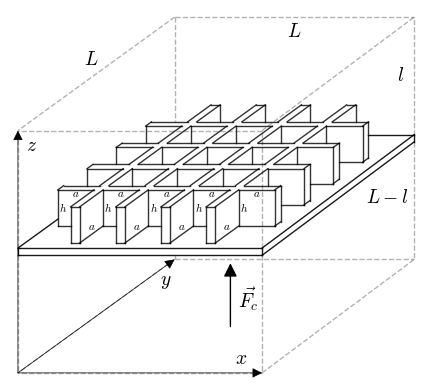
\includegraphics[width=0.42\textwidth]{honeycomb_box_H.png}
\caption{}{\centering{\textbf{Рис.1.} Кубічний резонатор із пластиною, вкритою стільниками.}}
\end{center}
\label{fig:honeycomb_box_H}
\end{figure}

Ідеально провідні стінки куба, як і в Казимира, --- допоміжна гранична умова без фізичного
прообразу, подібна до періодичних граничних умов, якими в підручниках квантової механіки нормують
плоскі хвилі. Процедура законна тому, що результат береться в границі \(L\to\infty\): за теоремою
Вейля \cite{Weyl1912} головний член кількості мод, \(N(k)\simeq Vk^3/3\pi^2\), не залежить від
граничних умов на зовнішніх гранях, від них залежать лише поверхневі поправки, і внесок віддалених
стінок у силу на пластину зникає. Обрізання \(k_m\) --- окремий, фізичний елемент: його задає
прозорість матеріалу пластини для коротких хвиль.

\vspace{\myvspacebeforesubsection}
\subsection*{\centering{\fontencoding{T2A}\fontfamily{ptm}{\selectfont ТЕОРЕМА НЕТЕР І НЕЗБЕРЕЖЕННЯ ІМПУЛЬСУ}}}
\vspace{\myvspaceaftersubsection}


Сума енергій нульових коливань \(E=\frac12\sum\hbar\omega\) за обома порожнинами дає вакуумний
гамільтоніан на одиницю площі \cite{Drozdov2024}:

\end{multicols}

\[
\frac{\langle 0|\hat{\mathcal{H}}|0\rangle}{S} = \frac{\hbar c}{a^2\pi} \Bigg\{
l \sum_{n_x=(0)1}^{\infty}\sum_{n_y=(0)1}^{\infty}
\int_0^{\infty} \sqrt{ \frac{\pi^2}{a^2}(n_x^2 + n_y^2) + k_z^2 } \, dk_z
+ (L - l) \int_0^{\infty}\!\!\int_0^{\infty}
\int_0^{\infty} \sqrt{k_x^2 + k_y^2 + k_z^2} \, dk_z \, \frac{a}{\pi}dk_x \frac{a}{\pi}dk_y
\Bigg\}.
\]

\begin{multicols}{2}

Цей вираз явно залежить від \(l\). Отже, система \textbf{не інваріантна} відносно нескінченно
малих трансляцій пластини \(z\to z+\delta z\).

За теоремою Нетер генератор просторових трансляцій --- компонента імпульсу \(P_z\) ---
зберігається \textbf{тоді й лише тоді}, коли гамільтоніан не залежить від \(z\). Оскільки
\(\partial\langle H\rangle/\partial l\neq0\), симетрію порушено, і \(P_z\) поля не зберігається.
Результуюча сила дорівнює

\end{multicols}

\[
\frac{F}{S} = \frac{\partial}{\partial l} \frac{\langle 0|\hat{\mathcal{H}}|0\rangle}{S}
= \frac{\hbar c}{a^2\pi} \left\{
\sum_{n_x=(0)1}^{\infty}\sum_{n_y=(0)1}^{\infty}
\int_0^{\infty} \sqrt{ \frac{\pi^2}{a^2}(n_x^2 + n_y^2) + k_z^2 } \, dk_z
- \int_0^{\infty}\!\!\int_0^{\infty}
\int_0^{\infty} \sqrt{k_x^2 + k_y^2 + k_z^2} \, dk_z \, dn_x dn_y
\right\},
\]

\begin{multicols}{2}

що збігається з формулою тяги, отриманою в \cite{Drozdov2024} через різницю густин енергії. Після
регуляризації \(f(k/k_m)\) і двовимірного підсумовування Ейлера--Маклорена вона набуває вигляду
\(F/S=\delta(E/V)=R(ak_m)\,\hbar c\,\pi/a^4\).

Отже, поява тяги не є несподіваною: це прямий наслідок порушеної трансляційної симетрії. Квантовий
вакуум «тисне» сильніше з одного боку, бо спектр мод з боків пластини різний. Одразу обумовимо,
про який імпульс ідеться: порушено трансляційну симетрію \emph{граничних умов}, а не простору.
Тому не зберігається імпульс поля --- або, що те саме, пластини, яка його поглинає; повний імпульс
системи \emph{пластина\,+\,поле\,+\,опора} зберігається, як у звичайного вітрила на вітрі. Де
саме поле передає імпульс пластині, покаже тензор натягів.

\vspace{\myvspacebeforesubsection}
\subsection*{\centering{\fontencoding{T2A}\fontfamily{ptm}{\selectfont ТЕНЗОР НАТЯГІВ З ПОЛІВ МОД}}}
\vspace{\myvspaceaftersubsection}


Обчислимо силу незалежно, через тензор натягів Максвелла, не припускаючи заздалегідь потоку
імпульсу плоскої хвилі. Явні поля TM- і TE-мод та перевірку рівнянь Максвелла й граничних умов
винесено в додаток~А. Одиниці гаусові, позначення Тамма \cite{Tamm1957}:
\(T_{ik}=\frac1{4\pi}(E_iE_k+H_iH_k)-\frac{\delta_{ik}}{8\pi}(E^2+H^2)\), сила на тіла всередині
замкненої поверхні дорівнює \(\oint T_{ik}n_k\,dS\), потік імпульсу \(\Pi_{ik}=-T_{ik}\). Нам
потрібна компонента
\[
T_{zz}=\frac1{8\pi}\left(E_z^2+H_z^2-E_x^2-E_y^2-H_x^2-H_y^2\right),
\]
тиск на горизонтальну площадку позначимо \(p\equiv-\langle T_{zz}\rangle\).

\textbf{Тиск однієї моди.} Усереднимо \(T_{zz}\) за перерізом \(ab\) і за періодом. За
\(n_x,n_y\ge1\) кожен множник \(\sin^2\) або \(\cos^2\) дає \(\tfrac12\), і для TM-моди
\[
8\pi\langle T_{zz}\rangle=\frac{A^2}{8}\left[\cos^2k_zz\left(1-\frac{k^2}{K^2}\right)-\frac{k_z^2}{K^2}\sin^2k_zz\right]
=-\frac{A^2}{8}\frac{k_z^2}{K^2},
\]
оскільки \(1-k^2/K^2=-k_z^2/K^2\). Густина енергії тієї самої моди, усереднена за об'ємом,
\(8\pi\overline w=\frac{A^2}{8}\frac{k^2}{K^2}\). Отже,
\[
p=-\langle T_{zz}\rangle=\overline w\,\frac{k_z^2}{k^2}.
\]
Для TE-моди ті самі кроки дають той самий результат. Якщо один із поперечних індексів дорівнює
нулю (це можливо лише для TE), загальний множник подвоюється і в тиску, і в енергії, відношення не
змінюється; TM-мода з \(n_z=0\) має \(k_z=0\) і тиску не створює.

\textbf{Незалежність від \(z\).} Залежність від \(z\) випала (\(\cos^2+\sin^2=1\)). Загальна
причина: у вакуумі \(\partial T_{zk}/\partial x_k=\frac1{4\pi c}\,\partial_t[\mathbf E\times\mathbf H]_z\),
а середнє за період від похідної за часом дорівнює нулю. Під час інтегрування за перерізом
залишаються потоки крізь бічні стінки \(T_{zx}=\frac1{4\pi}(E_zE_x+H_zH_x)\); на стінках
\(x=0,a\) \(E_z=0\) (дотичне поле) і \(H_x=0\) (нормальне), тобто \(T_{zx}=0\), і так само
\(T_{zy}=0\) на \(y=0,b\). Тому \(\frac{d}{dz}\int\langle T_{zz}\rangle\,dx\,dy=0\). Зазначимо:
від \(z\) не залежить лише інтеграл за перерізом; в окремій точці \((x,y)\) величина \(T_{zz}\)
змінюється із \(z\), але в силу входить саме інтеграл. Цей факт буде використано в наступному
розділі.

\textbf{Сума за нульовими коливаннями.} Кожна мода є осцилятором з енергією \(\hbar\omega/2\) в
основному стані, порівну розподіленою між електричною й магнітною частинами --- той самий
розподіл, що дає класичне усереднення за періодом, якщо покласти \(\overline w\,V=\hbar\omega/2\).
Тому тиск у порожнині
\[
p=\frac{\hbar c}{2V}\sum_{\text{моди}}\frac{k_z^2}{k}.
\]
Від суми для енергії \(E=\frac{\hbar c}{2}\sum k\) вона відрізняється лише доданком: \(k_z^2/k\)
замість \(k\).

\textbf{Тотожність із гамільтоновим підходом.} За \(k_z=\pi n_z/h\) маємо
\(\partial k/\partial h=-k_z^2/(kh)\), і для кожної моди
\[
-\frac{\partial}{\partial h}\frac{\hbar ck}{2}=\frac{\hbar c}{2h}\frac{k_z^2}{k}=S\,p_{\text{моди}},\qquad V=Sh .
\]
Сила, знайдена через тензор натягів, збігається з \(-\partial E/\partial h\) помодово, ще до
будь-якої регуляризації (теорема Гельмана--Фейнмана \cite{Feynman1939}; інакше кажучи, збереження
адіабатичного інваріанта \(E/\omega\) кожної моди за повільного зсуву стінки). Тим самим
гамільтонову силу попереднього розділу підтверджено незалежним методом.

\textbf{Виправлення додатка~B роботи \cite{Drozdov2024}.} Там тиск на грань \(xy\) обчислювався
як \(\langle H_x^2+H_y^2\rangle/8\pi\). Для TM-мод при цьому пропущено член
\(-\langle E_z^2\rangle/8\pi\): з ним відношення тиску до густини енергії дорівнює \(k_z^2/k^2\)
для мод обох типів, а не \(1\) для електричної моди (для моди \((2,1,3)\) за
\(a:b:h=1:1{,}3:2{,}7\) --- \(0{,}2119\) замість \(1\)). Тому значення \(1\) для електричної моди
і нерівність \(F/S\ge\delta(E/V)\) з \cite{Drozdov2024}, що на ньому ґрунтується, хибні.
Гамільтонове виведення додатка~C при цьому не зачіпається: за доведеною тотожністю воно помодово
збігається з тензорним.

\textbf{Регуляризація.} З обрізанням \(f(k/k_m)\) похідна енергії моди дорівнює
\(-\partial_h\!\left[\frac{\hbar ck}{2}f\right]=\frac{\hbar c}{2h}\frac{k_z^2}{k}\left[f+\frac{k}{k_m}f'\right]\),
а регуляризована тензорна сума \(\sum(k_z^2/k)f\) другого члена не містить. За скінченного
\(ak_m\) два вирази тому відрізняються, але за \(ak_m\to\infty\) відмінність зникає. Для
стільникової пластини це перевірено чисельно (розділ «Перевірки й оцінки»).

\textbf{Симетрійна перевірка.} Перенормований тензор \(\langle T_{\mu\nu}\rangle\)
електромагнітного поля безслідовий. Між двома паралельними пластинами граничні умови інваріантні
відносно бустів уздовж пластин; разом з умовою на слід це дає
\(\langle\Pi_{zz}\rangle=3\langle u\rangle\) (Браун і Маклей \cite{BrownMaclay1969}). Комірка
стільника --- хвилевід уздовж \(z\): далеко від торців її граничні умови інваріантні відносно
бустів уздовж \(z\), тому в блоці \((t,z)\) \(\langle T_{\mu\nu}\rangle\propto\eta_{\mu\nu}\) і
\(\langle\Pi_{zz}\rangle=-\langle u\rangle\), тобто \(|F/S|=\delta(E/V)\) --- те саме значення, що
дає гамільтонів підхід. Аргумент точний для ідеального провідника в границі \(ak_m\to\infty\) і з
точністю до торцевих поправок порядку \(a/l\).

\vspace{\myvspacebeforesubsection}
\subsection*{\centering{\fontencoding{T2A}\fontfamily{ptm}{\selectfont ДЕ ПРИКЛАДЕНА СИЛА}}}
\vspace{\myvspaceaftersubsection}


\textbf{Стрибок на поверхні металу.} На грані \(z=0\) (вакуум зовні, всередині металу поля дорівнюють
нулю) з боку вакууму \(E_x=E_y=0\), \(H_z=0\), тоді як нормальне \(\mathbf E\) і дотичне
\(\mathbf H\) зазнають стрибків \(4\pi\sigma\) і \(\frac{4\pi}{c}\mathbf i\). Тому
\[
T_{zz}\big|_{\text{вакуум}}=\frac1{8\pi}\left(E_z^2-H_x^2-H_y^2\right),\qquad
T_{zz}\big|_{\text{метал}}=0 .
\]
Для TM-моди за \(z=0\) \(\langle E_z^2\rangle=\frac{A^2}{8}\),
\(\langle H_x^2+H_y^2\rangle=\frac{A^2}{8}\frac{k^2}{K^2}\), звідки
\(-\langle T_{zz}\rangle(0^+)=\overline w\,k_z^2/k^2\) --- те саме значення, що в об'ємі порожнини;
для TE-моди \(E_z=0\) і результат той самий. Стрибок
\([\![T_{zz}]\!]=T_{zz}|_{\text{метал}}-T_{zz}|_{\text{вакуум}}=p\) є поверхневою силою на одиницю
площі, що діє на заряди \(\sigma=E_n/4\pi\) у полі \(E_n\) і на струми
\(\mathbf i=\frac{c}{4\pi}[\mathbf n\times\mathbf H]\) у полі \(\mathbf H_t\):
\[
\frac{f_z}{S}=\frac1{8\pi}\left(\langle H_t^2\rangle-\langle E_n^2\rangle\right).
\]
У вакуумному стані \(\langle\sigma\rangle=0\) і \(\langle\mathbf i\rangle=0\), але кореляції
\(\langle\sigma E_n\rangle\) і \(\langle\mathbf i\times\mathbf H\rangle\) відмінні від нуля: сила
квадратична за полями. Для TE-мод поверхневого заряду на гранях \(xy\) немає зовсім, і стрибок
створюють лише струми; це явний приклад стрибка тензора на поверхні, що не несе заряду.

Пластина має дві такі внутрішні межі: дно комірок і гладку грань. На кожній стрибок дорівнює тиску
прилеглої порожнини, \(p_{\text{cell}}=\frac{\hbar c}{2a^2l}\sum_{\text{комірка}}\frac{k_z^2}{k}\)
і \(p_{\text{big}}=\frac{\hbar c}{2L^2(L-l)}\sum_{\text{велика}}\frac{k_z^2}{k}\); всередині металу
\(T_{ik}=0\).

\begin{figure}
\begin{center}
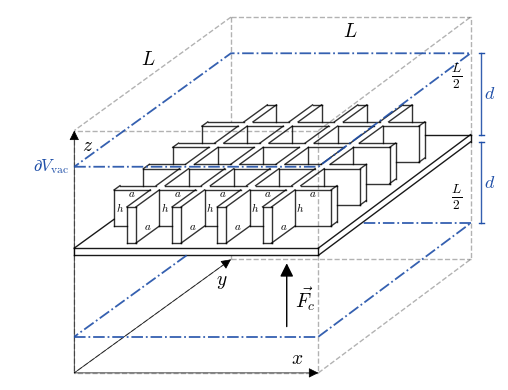
\includegraphics[width=0.42\textwidth]{honeycomb_box_L_d.png}
\caption{}{\centering{\textbf{Рис.2.} Грані «коробочки» \(\partial V_{\mathrm{vac}}\) при \(z=+d\) і \(z=-d'\).}}
\end{center}
\label{fig:honeycomb_box_L_d}
\end{figure}

\textbf{«Коробочка».} Охопимо пластину замкненою поверхнею \(\partial V_{\mathrm{vac}}\) з гранями
\(z=+d\) і \(z=-d'\) (\(0<d\le l\), \(0<d'\le L-l\)) на весь переріз \(L\times L\) (рис.~2);
бічні грані лежать на стінках куба, де \(T_{zx}=T_{zy}=0\). Тоді
\[
\begin{aligned}
F_z&=\oint_{\partial V_{\mathrm{vac}}}\langle T_{zz}\rangle\,da
=\left[\langle T_{zz}\rangle(d)-\langle T_{zz}\rangle(-d')\right]L^2\\
&=(p_{\text{big}}-p_{\text{cell}})\,L^2 .
\end{aligned}
\]
За доведеною незалежністю від \(z\) результат не залежить від \(d\), \(d'\). За \(d,d'\to0\) це
сума двох стрибків на гранях пластини --- сила прикладена до поверхонь металу; за \(d=l\),
\(d'=L-l\) грані підходять до допоміжних стінок куба (за \(l=L/2\) --- грані \(z=\pm L/2\)), що
розуміються як границя зсередини порожнин. На стільниковому боці грань перетинає стінки комірок;
за нульової товщини стінок вони внеску в інтеграл не дають. \(F_z>0\) (поштовх у бік комірок) за
\(p_{\text{big}}>p_{\text{cell}}\).

Потік крізь \(\partial V_{\mathrm{vac}}\) --- це потік імпульсу \emph{поля} крізь суто вакуумну
межу, а не сила, прикладена безпосередньо до речовини. Він відмінний від нуля лише тому, що спектр
мод, а отже й \(\langle T_{zz}\rangle\), різний на стільниковому і на гладкому боці.

\vspace{\myvspacebeforesubsection}
\subsection*{\centering{\fontencoding{T2A}\fontfamily{ptm}{\selectfont ЧОМУ СТАНДАРТНИЙ БАЛАНС ІМПУЛЬСУ ЦЬОГО НЕ БАЧИТЬ}}}
\vspace{\myvspaceaftersubsection}


Стандартне рівняння балансу імпульсу електродинаміки суцільних середовищ (Тамм, \S\,105
\cite{Tamm1957}) має вигляд

\end{multicols}
\[
\nabla\cdot\mathbf{T} = \frac{\partial\mathbf{g}}{\partial t} + \mathbf{f}_{\mathrm{vol}},
\qquad
\mathbf{g} = \frac{1}{c^2}\mathbf{S} = \frac{1}{4\pi c}[\mathbf{E}\times\mathbf{H}],
\]
\begin{multicols}{2}

де \(\mathbf{g}\) --- густина імпульсу поля, \(\mathbf{f}_{\mathrm{vol}}\) --- густина об'ємної
пондеромоторної сили. Для вакуумних флуктуацій статичної стільникової системи
\(\langle\mathbf{S}\rangle=0\), отже, \(\langle\partial\mathbf{g}/\partial t\rangle=0\). Якщо
ототожнити імпульс поля з \(\mathbf g\), то за \(\langle\mathbf S\rangle=0\) немає й перенесення
імпульсу --- і однотільна сила здається неможливою.

Перехід від об'ємних сил до натягів спирається на теорему Гаусса, яку Тамм застосовує (\S\,33,
ф.~33.7) за явної умови \emph{неперервності} компонент тензора натягів усередині об'єму; поверхні
розриву там виключено, а пізніше (\S\,34, ф.~34.8) розглядаються лише їхні поверхневі
\emph{заряди}. Але, як показано вище, межа вакуум--метал може не нести поверхневого заряду і все ж
давати скінченний стрибок тензора натягів. Цей випадок не розглянуто ні в \S\,33, ні деінде в книзі
Тамма, включно з \S\,105. Для об'єму \(V\), що містить внутрішні поверхні розриву \(S_j\), теорему
Гаусса треба записувати у вигляді

\end{multicols}
\[
\int_V \frac{\partial T_{ik}}{\partial x_k}\,dV
= \oint_{\partial V_{\mathrm{ext}}} T_{ik}\,n_k\,dS
\;-\; \sum_j \int_{S_j} [\![\,T_{ik}\,]\!]\,n_k\,dS_j ,
\]
\begin{multicols}{2}

де \([\![\cdot]\!]\) --- стрибок величини під час переходу крізь \(S_j\). Звичне ототожнення
імпульсу поля з \(\mathbf{g}=\mathbf{S}/c^2\) зберігає лише зовнішній поверхневий інтеграл і
втрачає стрибкові члени. Для стільникової пластини саме вони й становлять усю силу: сума двох
стрибків на гранях пластини дорівнює потоку крізь «коробочку».

Два зауваження роблять інтерпретацію однозначною. По-перше, як уже сказано, не зберігається імпульс
\emph{поля} (і пластини, що його поглинає), а не повний імпульс замкненої лабораторної системи.
По-друге, перенормований вакуумний натяг \(\langle T_{\mu\nu}\rangle\) є фізично вимірюваною
величиною --- це і є сам ефект Казимира, --- тому стрибкові члени не потребують припущення про
матеріальний ефір: їхнє значення задається тим самим \(\langle T_{\mu\nu}\rangle\), яке
підтверджено експериментально для симетричної конфігурації.

\vspace{\myvspacebeforesubsection}
\subsection*{\centering{\fontencoding{T2A}\fontfamily{ptm}{\selectfont ПЕРЕВІРКИ Й ОЦІНКИ}}}
\vspace{\myvspaceaftersubsection}


\textbf{Дві пластини Казимира.} Пластини за \(z=0\) і \(z=a\), зовнішні порожнини до
\(z=\pm L/2\). У зазорі \(k_z=\pi n/a\), поперечний спектр неперервний; на одиницю площі (дві
поляризації)
\[
p_{\text{in}}=\frac{\hbar c}{a}\sum_{n\ge1}\int\frac{d^2k_\parallel}{(2\pi)^2}\frac{k_z^2}{k},
\]
а зовні сума за \(n\) замінюється на \(\frac a\pi\int dk_z\). За незалежністю від \(z\) значення
\(p_{\text{in}}\) одне й те саме в центрі зазору й біля внутрішньої поверхні кожної пластини, а
\(p_{\text{out}}\) --- біля зовнішньої поверхні та на гранях \(z=\pm L/2\). З обрізанням
\(e^{-k/k_m}\) різниця \(p_{\text{in}}-p_{\text{out}}\) дорівнює \(-0{,}041043\), \(-0{,}041110\),
\(-0{,}041120\) в одиницях \(\hbar c/a^4\) за \(k_ma=20\), \(50\), \(100\) і прямує до
\(-\pi^2/240=-0{,}041123\). Знак означає притягання; з густиною енергії Казимира
\(u=-\pi^2\hbar c/720a^4\) це співвідношення \(p=3u\) \cite{BrownMaclay1969}.

\textbf{Тензорна сума для стільників.} Для стільникової пластини тензорну суму \(\sum k_z^2/k\) з
регулятором \(f=1/(1+k^4/k_m^4)\) обчислено тим самим двовимірним підсумовуванням, що й
енергетичну в \cite{Drozdov2024}. Позначимо \(D_E\) і \(D_T\) енергетичну й тензорну різниці «сума
мінус інтеграл». За малих \(ak_m\) вони відрізняються навіть знаком (член з \(f'\)), але за
\(ak_m=9\) і \(14\) отримано \(D_T+D_E=1\cdot10^{-4}\) і \(4\cdot10^{-6}\) відповідно за
\(|D_E|\approx0{,}012\): у границі \(ak_m\to\infty\) тензорне й гамільтонове виведення дають одну й
ту саму силу, \(|F/S|=\delta(E/V)\), у згоді з буст-аргументом.

\textbf{Оцінка тяги.} За \(\hbar c\,\pi/a^4=0{,}9932/a_\mu^4\)~дин/см\(^2\) (\(a_\mu\) --- сторона
комірки в мікронах) значення \(R=0{,}0138\) з таблиці~1 роботи \cite{Drozdov2024} дає для золотих
стільників з \(a\approx2\)~мкм \(F/S\approx8{,}55\)~дин/м\(^2\) \(=8{,}55\times10^{-5}\)~Н/м\(^2\).
Однак у \cite{Drozdov2024} ряд за оболонками \(j\) обривався, щойно черговий доданок ставав меншим
за поріг \(\epsilon\) (стовпці \(\epsilon\) і \(j_{max}\) таблиці~1). Хвостові доданки додатні й
спадають як \(j^{-3}\), тому відкинутий залишок
\(\epsilon\,j_{max}^3\,\zeta(3,j_{max}+1)\approx\epsilon\,j_{max}/2\) за малих \(ak_m\) мізерний,
а за \(ak_m=9\) (\(j_{max}=99\)) сягає \(15\%\). З цією поправкою таблиця~1 збігається з незалежним
перерахунком (замкнена форма інтеграла за \(u\), екстраполяція за розміром області підсумовування)
у межах \(0{,}13\%\) в усіх рядках. Виправлена границя \(|R|\approx0{,}0121\) відповідає
\(F/S\approx7{,}5\)~дин/м\(^2\). Порядок величини й висновок про практичну придатність для корекції
орбіт супутників від цього не змінюються.

\vspace{\myvspacebeforesubsection}
\subsection*{\centering{\fontencoding{T2A}\fontfamily{ptm}{\selectfont ОБМЕЖЕННЯ}}}
\vspace{\myvspaceaftersubsection}


(а) \textit{Висота комірок.} Розрахунок припускає, що стінки комірок доходять до грані куба і
комірка є замкненим резонатором. Для реальних комірок висотою \(h\ll L\) комірка відкрита у велику
порожнину, моди не розділяються, і цей розрахунок такого випадку не описує.

(б) \textit{Ідеальний провідник.} Стрибок є властивістю ідеального провідника. У реальному металі
\(T_{zz}\) спадає до нуля на товщині скін-шару, а інтеграл сили за шаром дорівнює стрибку, доки
струм у металі узгоджений з полем: \(\mathbf j=\frac c{4\pi}\nabla\times\mathbf H\).

(в) \textit{Товщина стінок.} Стінки комірок скінченної товщини не несуть \(z\)-сили (\(T_{zx}=0\)
на них), але зменшують частку площі пластини, зайняту порожнинами.

(г) \textit{Регуляризація.} Яка з двох регуляризованих величин --- енергетична чи тензорна ---
фізична за скінченного \(ak_m\), у моделі ідеального провідника з модовим обрізанням вирішити не
можна; для цього потрібна реальна \(\varepsilon(\omega)\), як у методі Дзялошинського, Ліфшиця й
Пітаєвського \cite{DLP1961}, де натяг у вакуумному зазорі знаходять із функції Гріна поля. Для
комірки стільника для цього потрібна функція Гріна прямокутного хвилеводу; це залишено для
подальшої роботи.

(д) \textit{Квантове середнє.} Рівність електричної й магнітної частин енергії моди в основному
стані використано як стандартний результат для осцилятора і тут не виводиться.

\vspace{\myvspacebeforesubsection}
\subsection*{\centering{\fontencoding{T2A}\fontfamily{ptm}{\selectfont ВИСНОВКИ}}}
\vspace{\myvspaceaftersubsection}


Стільниковий рушій Казимира є прикладом фізичної системи, у якій теорема Нетер безпосередньо
пояснює походження макроскопічної сили: \textbf{відсутність просторової однорідності призводить до
незбереження імпульсу поля}, а отже, до появи тяги. Незалежний розрахунок через тензор натягів
Максвелла, побудований з полів мод, відтворює ту саму силу --- помодово тотожно й після
регуляризації в границі \(ak_m\to\infty\), --- і при цьому виправляє помилку в додатку~B роботи
\cite{Drozdov2024}. Тензорний розрахунок показує, що сила прикладена до поверхонь металу у вигляді
стрибка \(\langle T_{zz}\rangle\), а стандартний баланс імпульсу \S\,105 Тамма, зведений до
\(\mathbf g=\mathbf S/c^2\), цих стрибкових членів не містить. Повний імпульс системи
\emph{пластина\,+\,поле\,+\,опора} зберігається. Експериментальна перевірка ефекту могла б
підтвердити зв'язок між геометрією граничних умов, симетрією і динамікою квантового вакууму.

\vspace{\myvspacebeforesubsection}
\subsection*{\centering{\fontencoding{T2A}\fontfamily{ptm}{\selectfont ДОДАТОК А. ПОЛЯ МОД}}}
\vspace{\myvspaceaftersubsection}


Поля TM-моди (\(H_z=0\), \(n_x,n_y\ge1\), \(n_z\ge0\)):
\end{multicols}
\[
\begin{aligned}
E_z&=A\sin k_xx\,\sin k_yy\,\cos k_zz\,\cos\omega t, &
H_z&=0,\\
E_x&=-A\frac{k_xk_z}{K^2}\cos k_xx\,\sin k_yy\,\sin k_zz\,\cos\omega t, &
H_x&=-A\frac{k\,k_y}{K^2}\sin k_xx\,\cos k_yy\,\cos k_zz\,\sin\omega t,\\
E_y&=-A\frac{k_yk_z}{K^2}\sin k_xx\,\cos k_yy\,\sin k_zz\,\cos\omega t, &
H_y&=A\frac{k\,k_x}{K^2}\cos k_xx\,\sin k_yy\,\cos k_zz\,\sin\omega t.
\end{aligned}
\]
Поля TE-моди (\(E_z=0\), \(n_z\ge1\), \((n_x,n_y)\ne(0,0)\)):
\[
\begin{aligned}
H_z&=A\cos k_xx\,\cos k_yy\,\sin k_zz\,\cos\omega t, &
E_z&=0,\\
H_x&=-A\frac{k_xk_z}{K^2}\sin k_xx\,\cos k_yy\,\cos k_zz\,\cos\omega t, &
E_x&=-A\frac{k\,k_y}{K^2}\cos k_xx\,\sin k_yy\,\sin k_zz\,\sin\omega t,\\
H_y&=-A\frac{k_yk_z}{K^2}\cos k_xx\,\sin k_yy\,\cos k_zz\,\cos\omega t, &
E_y&=A\frac{k\,k_x}{K^2}\sin k_xx\,\cos k_yy\,\sin k_zz\,\sin\omega t.
\end{aligned}
\]
\begin{multicols}{2}

Підстановкою перевіряється, що \(\nabla\cdot\mathbf E=\nabla\cdot\mathbf H=0\),
\(\nabla\times\mathbf E=-\frac1c\partial_t\mathbf H\), \(\nabla\times\mathbf H=\frac1c\partial_t\mathbf E\)
за \(\omega=ck\), і що виконано граничні умови ідеального провідника: дотичне \(\mathbf E\) і
нормальне \(\mathbf H\) перетворюються на нуль на всіх шести гранях (на \(x=0,a\): \(E_y=E_z=0\),
\(H_x=0\); на \(y=0,b\): \(E_x=E_z=0\), \(H_y=0\); на \(z=0,h\): \(E_x=E_y=0\), \(H_z=0\)). Ці
співвідношення перевірено символьно й чисельно для моди \((2,1,3)\) за \(a:b:h=1:1{,}3:2{,}7\).

Для TE-моди усереднення за перерізом і періодом дає
\(\langle H_z^2\rangle=\frac{A^2}{8}\sin^2k_zz\),
\(\langle H_x^2+H_y^2\rangle=\frac{A^2}{8}\frac{k_z^2}{K^2}\cos^2k_zz\),
\(\langle E_x^2+E_y^2\rangle=\frac{A^2}{8}\frac{k^2}{K^2}\sin^2k_zz\), звідки
\(8\pi\langle T_{zz}\rangle=-\frac{A^2}{8}\frac{k_z^2}{K^2}\) і \(p=\overline w\,k_z^2/k^2\).

\end{multicols}

\newpage

\fontencoding{T1}\fontfamily{ptm}\selectfont

\section*{\centering {\fontencoding{T1}\fontfamily{ptm}{\selectfont \uppercase{\mytitleen}}}}

\centerline{\Large{\mynameen \,\orcidlink{\myorcidlink} }}
\vspace{3mm}
\centerline{\textit{\myworkplaceen}}
\centerline{\textit{E-mail: \href{mailto:\myemail}{\myemail}}}

\vspace{3mm}
\centerline{\myreceiveden}
\centerline{\myaccepteden}

\vspace{3.5mm}

The Casimir honeycomb drive \cite{Drozdov2024} --- a perfectly conducting plate with a
nanoscale honeycomb structure on one side --- is examined from the standpoint of symmetries.
Because the vacuum modes on the two sides of the plate differ, the system is not invariant under
translations along the normal: the vacuum Hamiltonian depends explicitly on the coordinate \(l\),
and by Noether's theorem the field momentum along this axis is not conserved. The thrust equals
\(\partial\langle H\rangle/\partial l\). The same force is then computed independently, from the
Maxwell stress tensor built out of the fields of the cavity eigenmodes. Mode by mode the two
derivations coincide identically (Hellmann--Feynman theorem); after regularization they coincide
in the limit \(ak_m\to\infty\). Along the way an error in Appendix~B of \cite{Drozdov2024} is
found and corrected: for TM modes the ratio of pressure to energy density is \(k_z^2/k^2\), not
unity. The stress-tensor calculation shows where the force acts: it is the jump of
\(\langle T_{zz}\rangle\) at the metal surface, which is why the momentum flux through any closed
vacuum surface enclosing the plate is independent of the position of its faces. Finally, it is
shown that the standard momentum balance (Tamm, \S\,105) with \(\langle\mathbf S\rangle=0\) loses
exactly these jump terms. What is not conserved is the momentum of the field (and of the plate);
the total momentum of the system \emph{plate\,+\,field\,+\,support} is conserved.

\vspace{3mm}

\noindent
\textbf{\textit{Keywords:}} \textit{Noether's theorem, Casimir effect, quantum vacuum, momentum non-conservation, Maxwell stress tensor, nanohoneycomb, Casimir thrust}

\fontencoding{T2A}\fontfamily{ptm}\selectfont

\begin{thebibliography}{9}
\bibitem{Drozdov2024}
A. Drozdov, \textit{Casimir honeycomb drive: on the force on perfectly conducting honeycomb on a plate}, The Journal of V. N. Karazin Kharkiv National University. Series “Physics”, Iss. 41, 28--41 (2024). \url{https://doi.org/10.26565/2222-5617-2024-41-04}
\bibitem{Noether1918}
E. Noether, \textit{Invariante Variationsprobleme}, Nachr. d. König. Gesellsch. d. Wiss. zu Göttingen, Math-phys. Klasse, 235–257 (1918).
\bibitem{Casimir1948}
H. B. G. Casimir, \textit{On the attraction between two perfectly conducting plates}, Proc. K. Ned. Akad. Wet. B \textbf{51}, 793 (1948).
\bibitem{Tamm1957}
И. Е. Тамм, \textit{Основы теории электричества} (\S\,105, тензор натяжений Максвелла и баланс импульса электромагнитного поля), Наука, Москва.
\bibitem{Feynman1939}
R. P. Feynman, \textit{Forces in molecules}, Phys. Rev. \textbf{56}, 340 (1939).
\bibitem{BrownMaclay1969}
L. S. Brown, G. J. Maclay, \textit{Vacuum stress between conducting plates: an image solution}, Phys. Rev. \textbf{184}, 1272 (1969).
\bibitem{Weyl1912}
H. Weyl, \textit{Das asymptotische Verteilungsgesetz der Eigenwerte linearer partieller Differentialgleichungen}, Math. Ann. \textbf{71}, 441 (1912).
\bibitem{DLP1961}
И. Е. Дзялошинский, Е. М. Лифшиц, Л. П. Питаевский, \textit{Общая теория ван-дер-ваальсовых сил}, УФН \textbf{73}, 381 (1961).
\bibitem{VerifNotebook}
О. Дроздов, \textit{Перевірочні розрахунки до статті «Теорема Нетер та стільниковий рушій Казимира»}, Jupyter-ноутбук (SageMath 9.6), GitHub (2026). \url{https://github.com/daju1/articles/blob/master/casimir_noether/noether_casimir_verification.ipynb}
\end{thebibliography}

\end{document}
